\documentclass{article}
\usepackage[utf8]{inputenc}
\usepackage[T1]{fontenc}
\usepackage[french]{babel}
\usepackage{geometry}
\usepackage{graphicx}
\usepackage[hidelinks]{hyperref}
\usepackage{tocbibind} 
\usepackage{verbatim}
\usepackage{float}
\geometry{a4paper, margin=1in}

\title{Documentation sur le développement}
\date{30/11/2023}
\author{YANG Chen}
\begin{document}

\maketitle
\tableofcontents
\newpage

\begin{comment}
\section{Besoins du projet}
\subsection{Introduction}
Ce document vise à définir et décrire les besoins de développement de l'application de gestion de portefeuilles financiers. L'application offrira des outils pour créer, gérer et analyser des portefeuilles financiers personnels ou multiples, couvrant les investissements en actions et cryptomonnaies.

\subsection{Besoins Fonctionnels}
\subsubsection{Gestion de Portefeuille}
\begin{itemize}
    \item Création et gestion de portefeuille : Permettre aux utilisateurs de créer et de gérer plusieurs portefeuilles.
    \item Ajout/Suppression d'actifs : Soutenir l'ajout ou la suppression d'actions et de cryptomonnaies dans le portefeuille.
\end{itemize}

\subsubsection{Suivi des Données en Temps Réel}
\begin{itemize}
    \item Suivi de la valeur en temps réel : Afficher en temps réel la valeur de chaque actif dans le portefeuille.
    \item Consultation des données historiques : Fournir une fonction pour consulter la valeur et la performance du portefeuille à des moments passés.
\end{itemize}

\subsubsection{Intégration et Stockage des Données}
\begin{itemize}
    \item Intégration API : Obtenir des données en temps réel des marchés financiers via des API publiques.
    \item Importation de données : Permettre aux utilisateurs d'importer des données de plateformes de transactions externes (comme Coinbase ou Binance).
    \item Cache de données local : Pour améliorer la vitesse et l'efficacité d'accès, stocker les données localement.
\end{itemize}

\subsubsection{Interface Utilisateur}
\begin{itemize}
    \item Interface graphique : Offrir une interface intuitive et facile à utiliser.
    \item Visualisation des données : Présenter les actifs et la valeur du portefeuille sous forme de graphiques.
\end{itemize}

\subsection{Besoins Non Fonctionnels}
\subsubsection{Performance}
\begin{itemize}
    \item Réactivité rapide : Le temps de réponse de l'interface ne doit pas dépasser quelques secondes.
    \item Fréquence de mise à jour des données : La mise à jour des données financières ne devrait pas avoir plus d'une minute de retard.
\end{itemize}

\subsubsection{Sécurité}
\begin{itemize}
    \item Cryptage des données : Les données sensibles doivent être cryptées lors du stockage local.
    \item Sécurité d'accès : Nécessiter un mot de passe utilisateur pour accéder à l'application.
\end{itemize}

\subsection{Fonctionnalités Avancées}
\subsubsection{Fonctions d'Analyse}
\begin{itemize}
    \item Fournir des outils d'analyse de la performance des actifs et des portefeuilles.
    \item Encourager l'innovation et les fonctionnalités d'analyse personnalisées.
\end{itemize}

\subsubsection{Suivi des Transactions}
\begin{itemize}
    \item Suivre les transactions importantes sur la blockchain, en particulier les transactions de grande valeur (connues sous le nom de "traque des baleines").
\end{itemize}

\subsubsection{Choix de la Devise}
\begin{itemize}
    \item Permettre aux utilisateurs de choisir la devise de référence pour afficher la valeur des actifs (par exemple, EUR, USD, etc.).
\end{itemize}

\subsection{Besoins de l'Interface Utilisateur}
\begin{itemize}
    \item Intuitivité : L'interface doit être intuitive et facile à comprendre, simplifiant l'opération pour l'utilisateur.
    \item Personnalisation : Offrir une certaine mesure de personnalisation de l'interface et des options fonctionnelles.
\end{itemize}

\subsection{Contraintes Système}
\begin{itemize}
    \item Limitations techniques : L'application doit être compatible avec les systèmes d'exploitation et dispositifs principaux.
    \item Conformité légale : Respecter les lois et réglementations relatives aux données financières et à la vie privée.
\end{itemize}
\end{comment}

\section{Méthodologie de développement et gestion de projet}
\subsection{Spécification Du Code}
\begin{itemize}
    \item Langage de programmation : Java
    \item Style de codage 
    \subitem Suivez les conventions de code Java d'Oracle
    \subitem Utilisez une indentation appropriée (généralement quatre espaces)
    \item Structure du projet
    \subitem Suivez la structure standard des projets Maven
    \subitem Le code source est placé dans src/main/java et le code de test dans src/test/java
    \item Conventions de dénomination
    \subitem Les noms de classes et d'interfaces sont nommés en CamelCase
    \subitem Les noms de méthodes et de variables sont nommés en camelCase
    \subitem Les constantes sont séparées par des lettres majuscules et des traits de soulignement (par exemple, MAX\_VALUE)
    \item Spécification des annotations
    \subitem Utilisez Javadoc pour annoter les classes, les méthodes et les champs publics
    \subitem Utilisez des commentaires de ligne pour les segments de code logiques complexes
    \item Gestion des erreurs
    \subitem Préférez la gestion des exceptions au renvoi de codes d'erreur
    \subitem Les exceptions personnalisées doivent être claires et significatives
    \subitem Évitez les blocs catch vides
    \item Meilleures pratiques en matière de performances
    \subitem Évitez de créer des objets inutiles dans les boucles
    \subitem Utilisez des structures de données appropriées
    \subitem Optimisez les interactions avec les bases de données et les appels au réseau
    \item Spécification des tests
    \subitem Écrivez des tests unitaires qui couvrent les principales fonctionnalités et les conditions limites
    \subitem Utilisez JUnit ou d'autres cadres de test
    \item Contrôle de version
    \subitem Gérez le code à l'aide d'un système de contrôle de version tel que Github
    \subitem Suivez un processus clair de gestion des branches et de demande de fusion
\end{itemize}
\subsection{Choix du modèle en cascade}

Ce projet utilise le modèle en cascade comme méthodologie de développement logiciel. Le modèle en cascade est une méthode de développement séquentielle où chaque phase doit être complètement terminée avant de passer à la suivante. Ce modèle convient aux projets avec des objectifs clairs et des exigences stables.

Bien que notre équipe soit petite, composée de seulement deux membres, le choix du modèle en cascade est le plus approprié pour plusieurs raisons :
\begin{itemize}
    \item \textbf{Objectifs clairs du projet} : Les objectifs et les besoins du logiciel sont bien définis au début du projet.
    \item \textbf{Expérience des membres} : C'est la première participation de notre membre Remi et WenBin à un projet Java, donc une approche structurée et phasée aidera à une meilleure compréhension et participation. Toutefois, en raison de contraintes de temps, ils n'ont pas été en mesure de produire une documentation de bonne qualité, de sorte que la seconde moitié du projet a été modifiée pour adopter un modèle de développement agile.
\end{itemize}

\subsection{Planification du projet et chronologie}

Voici le plan détaillé du projet et la chronologie prévue :

\begin{itemize}
    \item \textbf{26 novembre 2023} - Lancement du projet
    \begin{itemize}
        \item Définition des objectifs et des exigences du projet.
        \item Discussion et détermination de la conception et de l'architecture de base du logiciel.
    \end{itemize}

    \item \textbf{1er décembre 2023} - Préparatifs initiaux
    \begin{itemize}
        \item Finalisation du document de besoins.
        \item Conception de l'architecture logicielle.
        \item Création de la structure du projet.
        \item Réalisation des diagrammes UML et des flux de processus métier.
    \end{itemize}

    \item \textbf{3 au 7 décembre 2023} - Création de classes et itération de la documentation
    \begin{itemize}
        \item Création de toutes les classes nécessaires selon le diagramme UML.
        \item Première itération de l'ensemble du document de développement pour assurer l'exactitude et l'exhaustivité de toutes les informations.
    \end{itemize}

    \item \textbf{10 au 14 décembre 2023} - Intégration et tests de l'API
    \begin{itemize}
        \item Finalisation de l'intégration avec les API externes.
        \item Réalisation de tests fonctionnels pour assurer la correcte intégration et la stabilité de l'API.
    \end{itemize}

    \item \textbf{17 au 22 décembre 2023} - Développement de la base de données et du frontend
    \begin{itemize}
        \item Construction de la base de données.
        \item Début du développement du frontend en JavaFx.
        \item Commencement du développement du backend.
        \item Deuxième itération du document de développement.
    \end{itemize}

    \item \textbf{25 décembre 2023 au 6 janvier 2024} - Développement du backend et tests
    \begin{itemize}
        \item Finalisation du développement du backend.
        \item Début des tests sur l'ensemble du système, incluant les tests unitaires et d'intégration.
    \end{itemize}

    \item \textbf{8 au 12 janvier 2024} - Finalisation des tests et préparation du lancement
    \begin{itemize}
        \item Achèvement de tous les travaux de test pour assurer la stabilité et la performance du logiciel.
        \item Préparation du lancement du logiciel, incluant la documentation finale pour les utilisateurs et le guide de déploiement.
    \end{itemize}
\end{itemize}

\subsection{Remarques}

\begin{itemize}
    \item Comme nous utilisons le modèle en cascade, la transition entre les phases est cruciale. À la fin de chaque phase, une revue complète et une mise à jour de la documentation sont nécessaires.
    \item Il est essentiel de surveiller attentivement la chronologie du projet pour s'assurer que chaque phase est complétée à temps. Tout problème susceptible d'affecter le calendrier doit être signalé et résolu immédiatement.
\end{itemize}

\section{Environnement et outils de développement}
\begin{itemize}
    \item Système d'exploitation : MacOS Ventura 13.4 \& Windows 11
    \item IDE : Visual Studio Code \& IntelliJ IDEA
    \item Langage de programmation : Java 19.0.2
    \item Cadre Back-End : Spring boot 2.7.0
    \item Cadre Front-End : JavaFx 17.0.1
    \item Base de données : Simuler le stockage d'une base de données à l'aide de fichiers json
    \item Autre : Maven \& GitHub \& Draw.io \& LaTex
\end{itemize}
\section{Technologie d'architecture et de conception}


\subsection{Architecture logicielle de haut niveau}

Ce projet adopte le modèle d'architecture MVC (Modèle-Vue-Contrôleur) et est étendu par une couche de gestion des services et une couche d'accès aux données. Le but de cette architecture est de réaliser une séparation des préoccupations, rendant ainsi le système plus facile à maintenir et à mettre à jour. Dans ce projet, la couche Service est principalement responsable du traitement de la logique métier. Cette couche est conçue pour gérer des opérations commerciales complexes, assurant ainsi la clarté et la maintenabilité du code. En même temps, la couche Modèle joue principalement le rôle de porteur de données dans ce projet. La simplification de la couche Modèle rend la structure des données du système plus intuitive et facilite également l'interaction avec la source de données. La couche Vue est responsable de la présentation des données, tandis que la couche Contrôleur coordonne l'interaction entre le modèle et la vue.
\subsubsection{Choix de la Pile Technologique}
Pour la partie backend du projet, nous avons choisi le framework SpringBoot, tandis que le frontend utilise JavaFX. SpringBoot, en tant que framework backend largement utilisé, offre des avantages tels que le développement rapide, la facilité de configuration et un solide soutien communautaire. Cependant, en raison des caractéristiques du cycle de vie des composants JavaFX, leur intégration directe avec SpringBoot présente des défis. Pour résoudre ce problème, nous avons apporté des modifications adaptatives à la structure du projet pour assurer la compatibilité entre les deux. Pour plus de détails sur les modifications, veuillez consulter le document technique.
\subsubsection{Caractéristiques Clés de SpringBoot}
\begin{enumerate}
    \item Démarrage Rapide et Configuration Automatique
    \begin{itemize}
        \item La fonction de démarrage rapide de SpringBoot réduit considérablement le cycle de développement, nous permettant d'entrer plus rapidement dans la phase principale du développement. De plus, le mécanisme de configuration automatique de SpringBoot simplifie la configuration du projet, en configurant automatiquement le conteneur Spring et les dépendances, réduisant ainsi la complexité de la configuration et améliorant l'efficacité du développement.
    \end{itemize}
    \item Injection de Dépendances
    \begin{itemize}
        \item Le mécanisme d'injection de dépendances de SpringBoot est particulièrement bénéfique pour les tests unitaires et d'intégration ultérieurs. Ce mécanisme réduit le couplage entre les composants, facilitant ainsi les tests unitaires. L'injection de dépendances améliore non seulement la modularité du code, mais rend également les tests plus faciles à réaliser et à maintenir, assurant ainsi la qualité du code et la stabilité du système.
    \end{itemize}
\end{enumerate}





\begin{comment}
    \subsubsection{Modèle (Model)}
La couche modèle constitue le cœur de l'architecture logicielle. Elle encapsule la logique métier et les structures de données, gérant les interactions avec la base de données et l'exécution des règles métier. Les entités au sein du dossier \texttt{model} représentent les objets du domaine tels que les comptes financiers, les transactions et les portefeuilles d'investissement.

\subsubsection{Vue (View)}
La couche vue est chargée de l'affichage des données à l'utilisateur et de la gestion des interactions utilisateur. Elle est construite en utilisant JavaFX pour offrir une expérience utilisateur graphique riche et interactive. Les éléments dans le dossier \texttt{view} sont des composants graphiques qui présentent les données et réagissent aux actions de l'utilisateur.

\subsubsection{Contrôleur (Controller)}
Les contrôleurs servent de médiateurs entre la vue et le modèle. Ils interprètent les entrées de l'utilisateur, invoquent des changements sur le modèle et sélectionnent la vue appropriée pour la réponse. Le dossier \texttt{controller} contient la logique de navigation et de coordination des flux d'utilisation.

\subsubsection{Couche de services (Service)}
La couche de services offre une abstraction de la logique métier, exposant un ensemble de services de haut niveau utilisés par les contrôleurs. Elle facilite la réutilisation du code métier et décore le modèle avec des opérations complexes. Le dossier \texttt{service} encapsule les processus métier tels que l'analyse financière et la synchronisation des données.

\subsubsection{Accès aux données (Repository)}
La couche d'accès aux données abstrait la persistance et la récupération des données. Elle fournit une interface pour interagir avec les sources de données, garantissant l'isolation entre la logique métier et les détails de la base de données. Le dossier \texttt{repository} implémente les interactions avec la base de données.

\subsubsection{Configuration (Config)}
La configuration de l'application est gérée dans la couche de configuration. Elle inclut les paramètres de démarrage, les configurations de la base de données, les clés API pour les services externes et les détails de l'injection de dépendance. Le dossier \texttt{config} contient des classes de configuration et du code d'initialisation.

Chaque couche est conçue pour être indépendante mais interopérable, permettant une division claire des responsabilités et une évolution simplifiée du système.
\end{comment}


\subsection{Interaction du système}

\subsubsection{vue d'ensemble du système}

L'application de gestion de portefeuille est une solution complète conçue pour permettre aux utilisateurs de gérer efficacement leurs investissements, qu'il s'agisse d'actions, de crypto-monnaies ou de transactions financières. Son objectif principal est de fournir une interface utilisateur simple, intuitive et performante permettant à l'utilisateur de visualiser, analyser et effectuer des actions liées à son portefeuille financier.
L'application prend en charge la gestion de divers types d'actifs, notamment :
\begin{itemize}
    \item les actions : l'application permet de suivre, d'acheter ou vendre des actions.
    \item les crypto-monaies : l'application donne la possibilité à l'utilisateur de suivre les variations de prix des crypto-monnaies, d'acheter ou de vendre des crypto-monnaies
    \item les transactions : l'application permet de gérer des transactions financières liées aux actions et aux crypto-monnaies, offrant ainsi une vue détaillée de l'historique des transactions.
    \item la gestion de porte-feuilles : ajouter, cloner et visualiser ce que contient les porte-feuilles de l'utilisateur.
\end{itemize}

\subsubsection{architecture et conception}

L'application repose sur une architecture robuste, utilisant des modèles de conception tels que MVC (Modèle-Vue-Contrôleur) pour assurer une séparation claire des responsabilités. Elle peut être intégrée à des services externes (API) pour fournir des informations en temps réel sur les actions et les crypto-monnaies.

\begin{itemize}
    \item Model : Le modèle est responsable de la gestion des données, de la logique métier et des interactions avec la base de données. Il comprend des classes telles que : 
    
    - Asset
    
    - Market
    
    - marketTransactoin
    
    - Portfolio
    
    - Transaction
    
    - User
    
\end{itemize}

\subsubsection{Conception de l'interface utilisateur}

L'interface utilisateur est organisée de manière à fournir une navigation claire et à permettre un accès rapide aux fonctionnalités principales de l'application. Le composant clé de l'application est le menu à partir duquel l'utilisateur peut accéder à toutes les fonctionnalité de l'application après s'être identifier ou après avoir créé un compte.
dans le menu, l'utilisateur peut avoir accès à :
\begin{itemize}
    \item la liste et la gestion de ses portefeuilles (évolution des porte-feuilles, création de nouveaux, clonage de porte-feuilles)
    \item liste et gestion des actions (cours avec API, vente, achat)
    \item liste et gestion des crypto-monnaies (cours avec API, vente, achat)
    \item gestion des transactions (virement)
\end{itemize}

\subsubsection{Flux d'interaction}

Les flux d'interactions de l'application de gestion de portefeuille décrivent comment les utilisateurs interagissent avec le système pour effectuer diverses actions liées à la gestion de leurs actifs financiers. Ces interactions englobent l'ajout d'actifs, la gestion de portefeuilles, l'exécution de transactions, et la visualisation des performances. Voici un aperçu non exhaustif des principaux flux d'interactions :

\begin{itemize}
    \item gestion des porte-feuilles
    \item ajout ou vente d'actif
    \item ajout ou vente de crypto-monnaies
    \item exécution de transaction
    \item visualisation des performances
    
\end{itemize}
\subsection{Considérations de sécurité et de performance}
\subsubsection{Considérations sur la Sécurité}
Dans ce projet, nous avons adopté une méthode de stockage de données locale pour les utilisateurs, spécifiquement au format de fichier JSON. Afin d'assurer la sécurité des données, toutes les informations sensibles ont été cryptées. La méthode de cryptage spécifique et les détails sont décrits en détail dans le document technique. Prenant l'exemple du mot de passe utilisateur, en tant que partie des informations sensibles, il est toujours stocké localement sous forme cryptée pour garantir la sécurité.
\subsubsection{Considérations sur la Performance}
En termes de performance, nous avons remarqué que le volume de lecture et d'écriture des données dans le projet actuel n'est pas important. Sur cette base, nous avons développé un ensemble d'outils personnalisés pour la lecture et l'écriture de documents. Cet outil, en implémentant les fonctionnalités de sérialisation et de désérialisation de la bibliothèque Jackson, permet une lecture et une écriture efficaces des fichiers. Pour plus de détails sur la mise en œuvre, veuillez consulter le document technique.

Étant donné que les membres de l'équipe, Remi et Wenbin, ne sont pas encore familiers avec les principes de la programmation asynchrone, nous n'avons pas utilisé de méthodes asynchrones dans le projet actuel. Cela signifie que toutes les opérations documentaires sont thread-safe.
\subsubsection{Développement Piloté par Événements}
Compte tenu de la manipulation de fichiers locaux, de la gestion des données en mémoire et des mises à jour de l'interface utilisateur (UI) impliquées dans le projet, nous avons choisi le modèle de développement piloté par événements pour optimiser le traitement de ces aspects. Le développement piloté par événements offre un mécanisme efficace pour faire face aux divers événements liés aux opérations de fichier et aux mises à jour de l'UI. Pour plus de détails sur le développement piloté par événements, veuillez consulter le document technique.
\subsection{Diagramme de processus métier}
\begin{figure}[H]
    \centering
    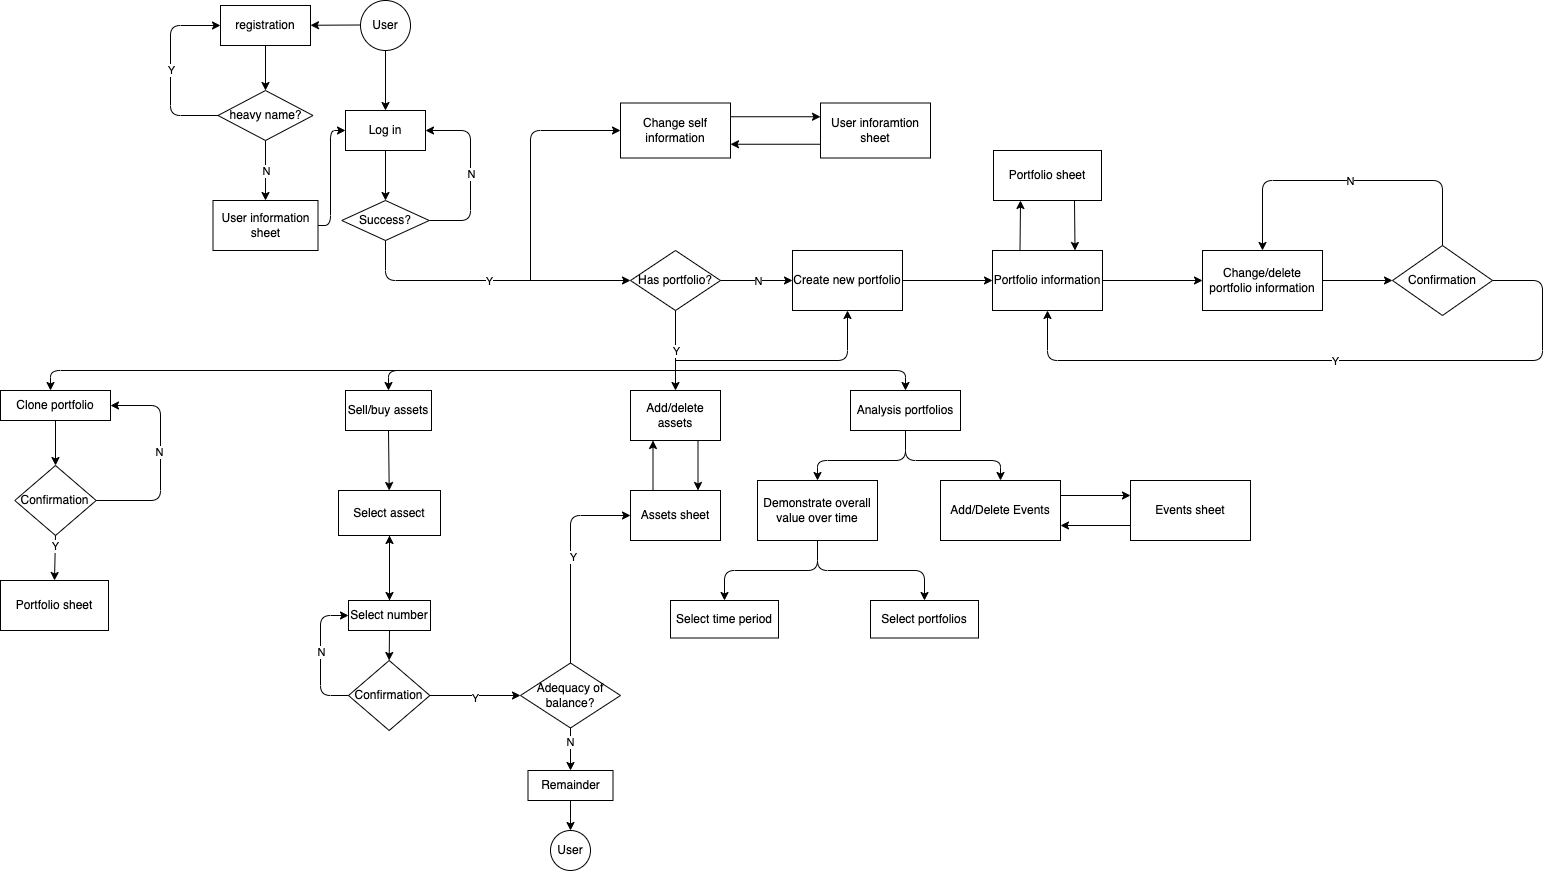
\includegraphics[width=0.7\textwidth]{../analysises/bussness process/V1.0/analysisV1.0.png}
    \caption{Diagramme de processus métier}
    \label{fig:processusMetier}
\end{figure}
\subsection{Diagramme de UML}
\begin{figure}[H]
    \centering
    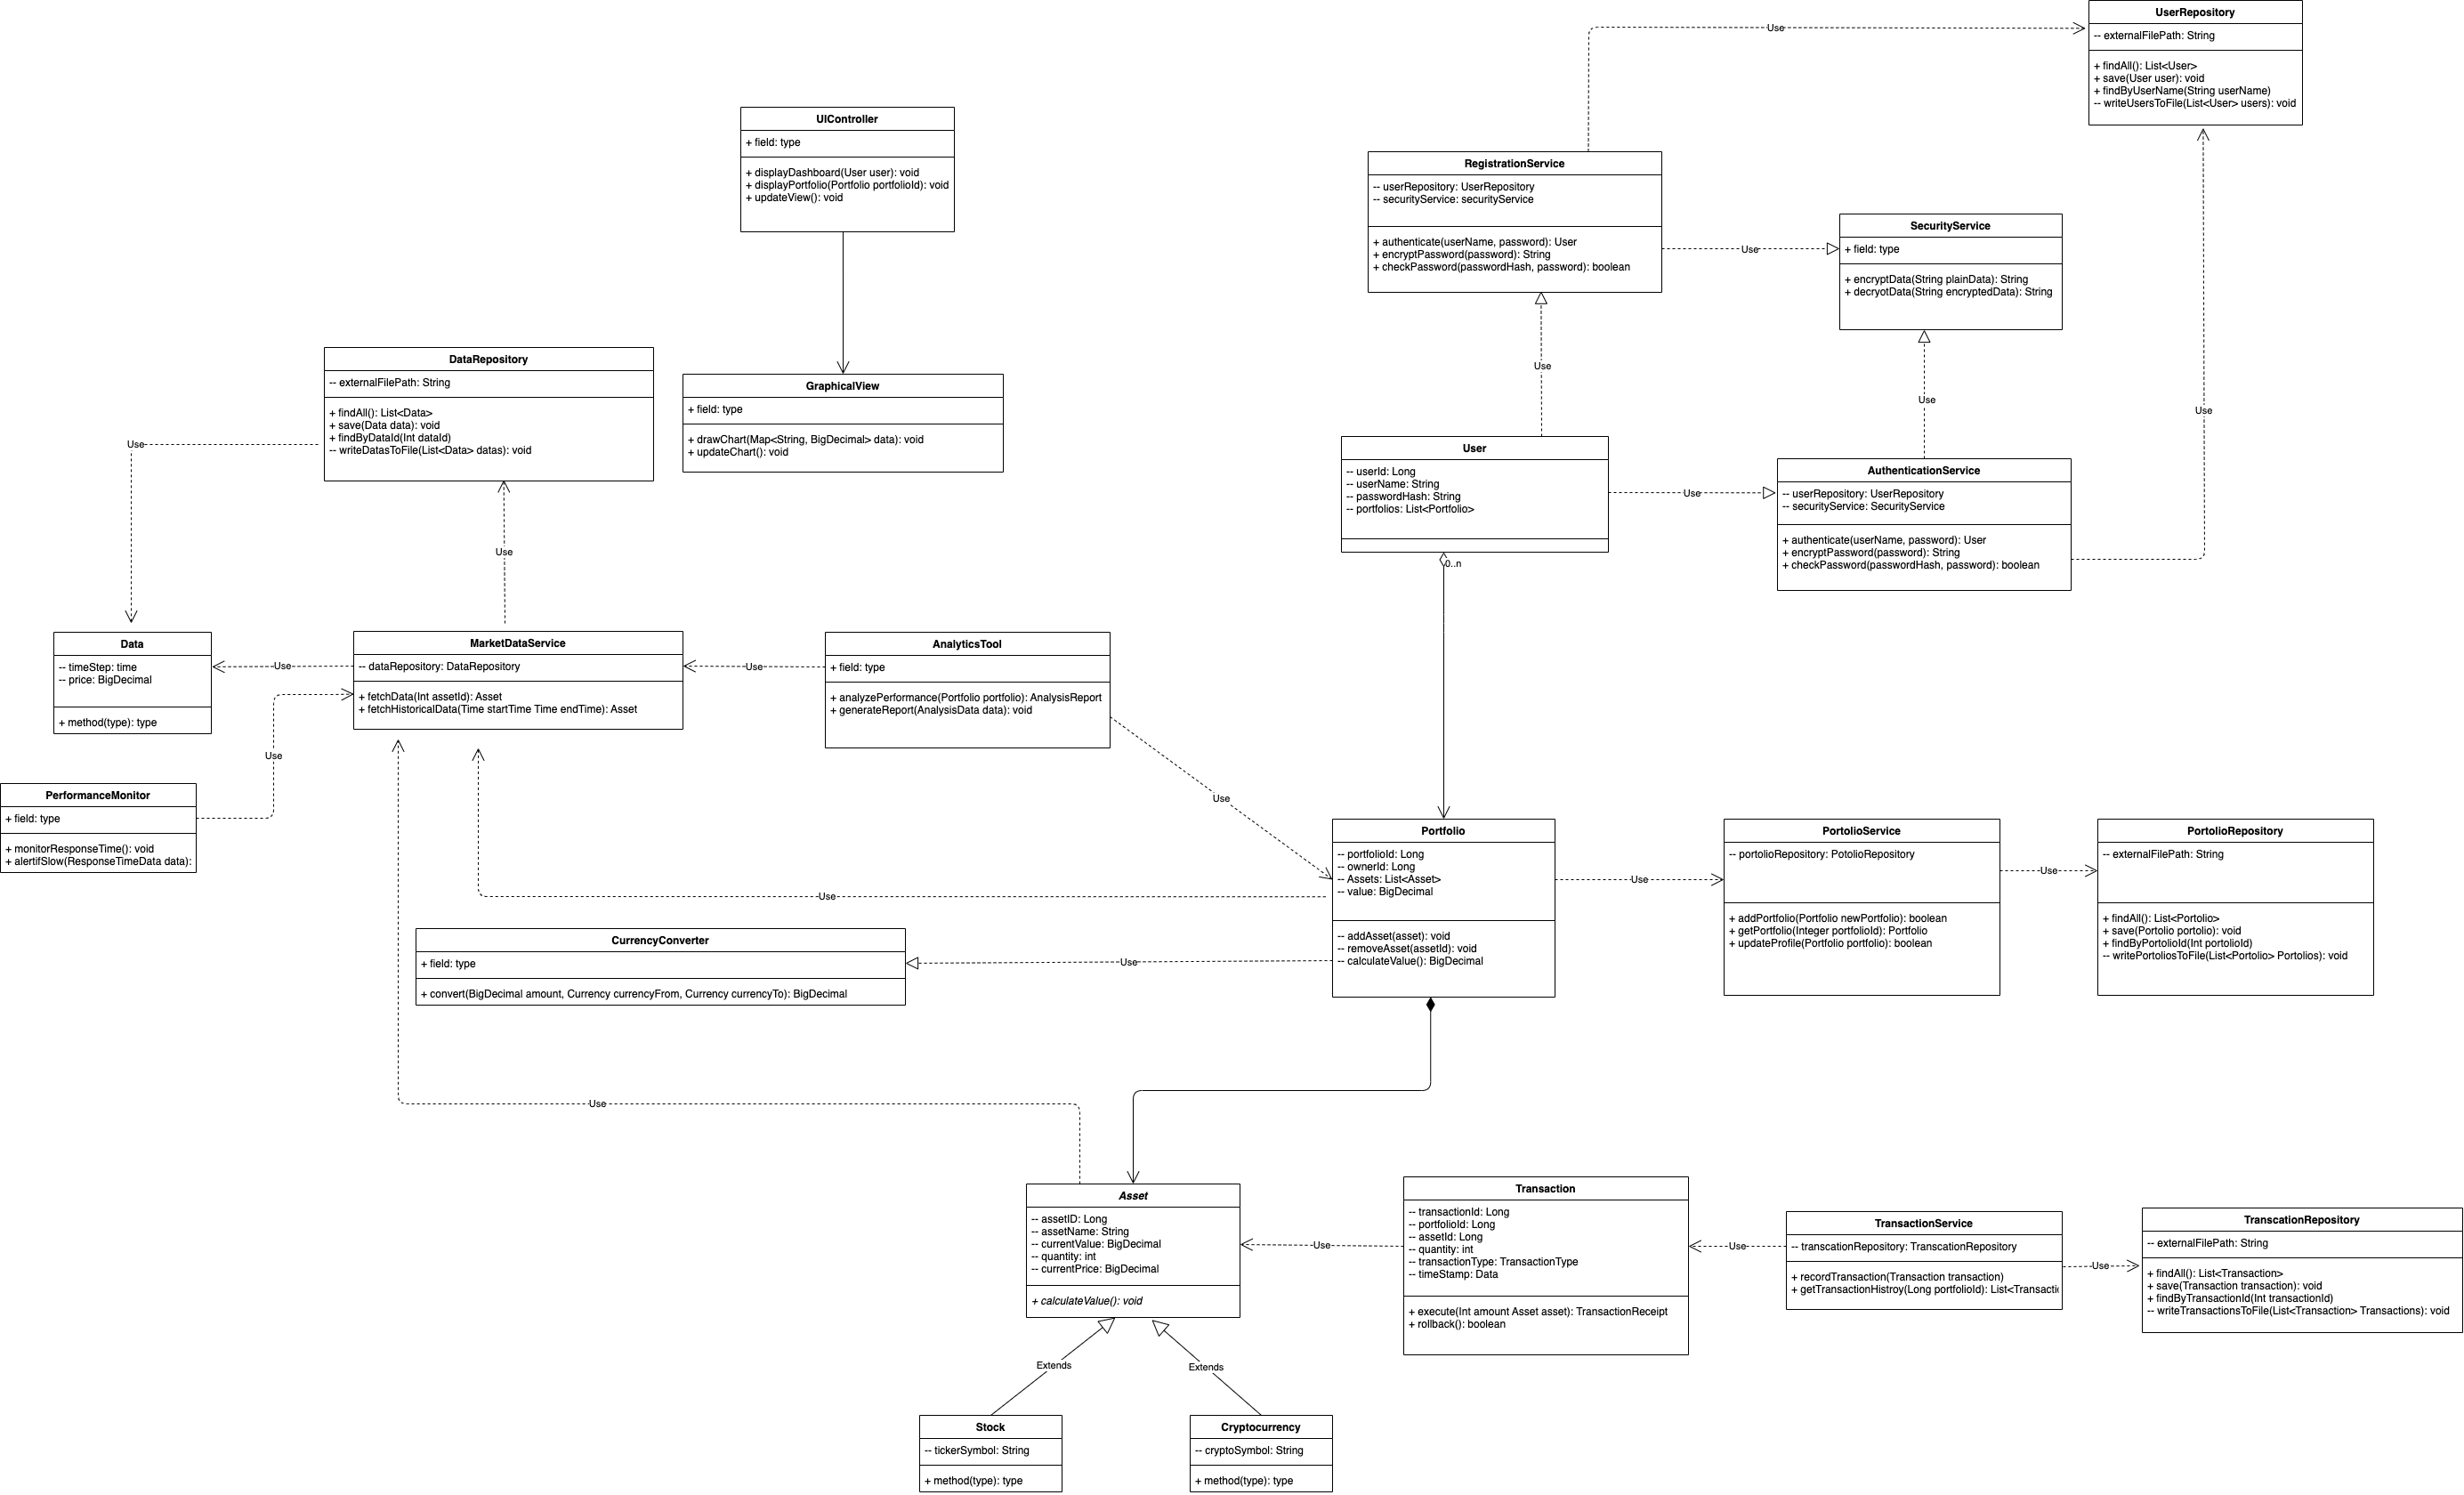
\includegraphics[width=0.7\textwidth]{../analysises/UML/V1.0/UMLV1.4.png}
    \caption{Diagramme de UML}
    \label{fig:UML}
\end{figure}

\subsection{Application des Modèles de Conception}
\subsubsection{Méthode de la Fabrique}
Dans ce projet, le modèle de conception de la méthode de la fabrique est utilisé pour créer différents types d'actifs. Nous avons plusieurs types d'actifs, tels que l'espèce et les dépôts à terme, qui héritent tous de la classe Asset. Les dépôts à terme, en tant que type spécial d'actif, nécessitent des paramètres supplémentaires tels que le taux d'intérêt pour être instanciés. La méthode de la fabrique nous permet de créer différents types d'objets d'actifs selon les besoins, sans exposer la logique spécifique de leur création. Ce modèle offre un moyen flexible d'étendre les types d'actifs tout en maintenant la clarté et la maintenabilité du code.
\subsubsection{Modèle Singleton}
Le modèle Singleton est largement appliqué dans cette application. Dans notre conception, le programme permet à un seul utilisateur de se connecter et d'utiliser l'application à tout moment. Chaque utilisateur ne peut accéder et opérer qu'un seul portfolio et un seul actif à la fois. De plus, pour chaque portfolio en cours d'opération, il n'y a qu'une seule instance de la classe Cash dans le système. Le modèle Singleton est très approprié ici, car il assure qu'il n'y a qu'une seule instance globale, ce qui aide à éviter les conflits et les incohérences sur les ressources partagées. En même temps, cela simplifie la gestion des ressources et le contrôle d'accès, assurant la stabilité du programme et la cohérence des données.
\subsubsection{Raison pour Ne Pas Utiliser le Modèle Observateur}
Bien que notre programme adopte une architecture pilotée par événements pour les mises à jour de l'UI et des données, nous avons choisi de ne pas utiliser le modèle observateur. Cela est principalement dû au fait que dans le contexte spécifique de notre projet actuel, l'architecture pilotée par événements est suffisante pour gérer efficacement les mises à jour synchronisées de l'UI et des données. Bien que le modèle observateur puisse offrir un contrôle de mise à jour plus fin dans certains scénarios, il peut également introduire des dépendances plus complexes et des coûts de maintenance plus élevés. Dans notre cas, la méthode simplifiée pilotée par événements répond déjà aux besoins, tout en conservant la simplicité et l'efficacité du système.



\begin{comment}
    \section{Conception détaillée}
\subsection{Service}
\subsubsection{Registration Service (Service d'Enregistrement)}
\paragraph{Responsabilités:} Traite la logique d'enregistrement des nouveaux utilisateurs.
\paragraph{Méthodes:}
\begin{itemize}
  \item \textbf{register}(userName: String, password: String, passwordEnsurance: String): RegistrationResult
\end{itemize}
\paragraph{Exceptions:}
\begin{itemize}
  \item \textbf{IOException} : Si le fichier de stockage des utilisateurs n'est pas accessible. 
\end{itemize}
\subsubsection{Authentication Service (Service d'Authentification)}
\paragraph{Responsabilités:} Traite la logique d'authentification des utilisateurs.
\paragraph{Méthodes:}
\begin{itemize}
  \item \textbf{authenticate}(userName: String, password: String): AuthenticationResult
  \item \textbf{checkPassword}(passwordHash: String, password: String): Boolean
\end{itemize}
\subsubsection{Security Service (Service de Sécurité)}
\paragraph{Responsabilités:} Gère les opérations de sécurité et d'autorisation.
\paragraph{Méthodes:}
\begin{itemize}
  \item \textbf{encryptData}(plainData: String): String
  \item \textbf{decryptData}(encryptedData: String): String
\end{itemize}
\subsubsection{Portfolio Service (Service de Portefeuille)}
\paragraph{Responsabilités:} Gère les services de portefeuille d'investissement.
\paragraph{Méthodes:}
\begin{itemize}
  \item \textbf{getPortfolio}(portfolioId: int): Portfolio
  \item \textbf{updatePortfolio}(portfolio: Portfolio): Boolean
  \item \textbf{addPortfolio}(portfolio: Portfolio): Boolean
  \item \textbf{createPortfolio}(portfolioName : String, ownerId: int): Portfolio
\end{itemize}
\subsubsection{Asset Service (Service d'Actif)}
\paragraph{Responsabilités:} Gère les services d'actif.
\paragraph{Méthodes:}
\begin{itemize}
  \item \textbf{getAsset}(assetId: int): Asset
  \item \textbf{updateAsset}(asset: Asset): Boolean
  \item \textbf{addAsset}(asset: Asset): Boolean
  \item \textbf{createAsset}(assetName: String, portfolioId: int, quantity: int,
  price: BigDecimal, assetType: ASSET\_TYPE,  interestRate: BigDecimal): Asset
\end{itemize}

\subsubsection{Transaction Service (Service de Transaction)}
\paragraph{Responsabilités:} Gère la logique des transactions.
\paragraph{Méthodes:}
\begin{itemize}
  \item \textbf{recordTransaction}(transaction: Transaction): void
  \item \textbf{getTransactionHistory}(portfolioId: int): List<Transaction>
\end{itemize}
\subsubsection{Market Data Service (Service des Données du Marché)}
\paragraph{Responsabilités:} Fournit des services de données de marché.
\paragraph{Méthodes:}
\begin{itemize}
  \item \textbf{fetchData}(assetId: int): List<Asset>
  \item \textbf{fetchHistoricalData}(startTime: Time, endTime: Time): List<Asset>
\end{itemize}
\paragraph{Exceptions:}
\begin{itemize}
  \item \textbf{IOException} : Si l'API externe est inaccessible.
\end{itemize}
\subsection{Repository}
\subsubsection{User Repository (Dépôt Utilisateur)}
\paragraph{Responsabilités:} Gère le stockage et la récupération des données utilisateur.
\paragraph{Méthodes:}
\begin{itemize}
  \item \textbf{findAll}(): List<User>
  \item \textbf{save}(user: User): Boolean
  \item \textbf{findByUserName}(userName: String): User
\end{itemize}

\subsubsection{Data Repository (Dépôt de Données)}
\paragraph{Responsabilités:} Gère le stockage et la récupération des données d'application.
\paragraph{Méthodes:}
\begin{itemize}
  \item \textbf{findAll}(): List<Asset>
  \item \textbf{save}(Data: data): Boolean
  \item \textbf{findByDataTimeStamp}(dataTimeStamp: Time): Data
  \item \textbf{findByDataTimeStamp}(startTime: Time, endTime: Time): List<Data>
\end{itemize}
\subsubsection{Transaction Repository (Dépôt de Transaction)}
\paragraph{Responsabilités:} Gère le stockage et la récupération des données de transaction.
\paragraph{Méthodes:}
\begin{itemize}
  \item \textbf{findAll}(): List<Transaction>
  \item \textbf{save}(transaction: Transaction): Boolean
  \item \textbf{findByPortfolioId}(portfolioId: int): List<Transaction>
\end{itemize}
\subsubsection{Portfolio Repository (Dépôt de Portefeuille)}
\paragraph{Responsabilités:} Gère le stockage et la récupération des données de portefeuille d'investissement.
\paragraph{Méthodes:}
\begin{itemize}
  \item \textbf{findAll}(): List<Portfolio>
  \item \textbf{save}(portfolio: Portfolio): Boolean
  \item \textbf{findByPortfolioId}(portfolioId: int): Portfolio
\end{itemize}
\subsubsection{Asset Repository (Dépôt d'Actif)}
\paragraph{Responsabilités:} Gère le stockage et la récupération des données d'actif.
\paragraph{Méthodes:}
\begin{itemize}
  \item \textbf{findAll}(): List<Asset>
  \item \textbf{save}(asset: Asset): Boolean
  \item \textbf{findByAssetId}(assetId: int): Asset
  \item \textbf{findByOwnerId}(ownerId: int): List<Asset>
\end{itemize}
\subsection{Model}
\subsubsection{Analytics Tool (Outil d'Analyse)}
\paragraph{Responsabilités:} Fournit des outils d'analyse de données.
\subsubsection{Performance Monitor (Surveillance de la Performance)}
\paragraph{Responsabilités:} Surveille la performance du Service des Données du Marché pour déterminer si l'API externe est trop lente.
\subsubsection{User (Utilisateur)}
\paragraph{Responsabilités:} Représente un utilisateur.
\paragraph{Propriétés:}
\begin{itemize}
  \item \textbf{userName}: String
  \item \textbf{userId}: int
  \item \textbf{passwordHash}: String
  \item \textbf{portfolios}: List<Portfolio>
\end{itemize}
\subsubsection{Data (Donnée)}
\paragraph{Responsabilités:} Représente une donnée collecté.
\paragraph{Propriétés:}
\begin{itemize}
  \item \textbf{price}: BigDecimal
  \item \textbf{timeStamp}: Time
\end{itemize}
\subsubsection{Authentication Result (Résultat d'Authentification)}
\paragraph{Responsabilités:} Représente le résultat d'une tentative d'authentification.
\paragraph{Propriétés:}
\begin{itemize}
  \item \textbf{sucess}: Boolean
  \item \textbf{failureType}: AUTHENTICATION\_FAILIURE\_TYPE
  \item \textbf{user}: User
\end{itemize}
\subsubsection{Registration Result (Résultat d'Inscription)}
\paragraph{Responsabilités:} Représente le résultat d'une tentative d'inscription.
\paragraph{Propriétés:}
\begin{itemize}
  \item \textbf{sucess}: Boolean
  \item \textbf{failureType}: REGISTRATION\_FAILIURE\_TYPE
  \item \textbf{user}: User
\end{itemize}
\subsubsection{Portfolio (Portefeuille)}
\paragraph{Responsabilités:} Représente un portefeuille d'investissement.
\paragraph{Propriétés:}
\begin{itemize}
  \item \textbf{portfolioId}: int
  \item \textbf{ownerId}: int
  \item \textbf{assets}: List<Asset>
\end{itemize}
\subsubsection{Asset (Actif)}
\paragraph{Responsabilités:} Représente un actif.
\paragraph{Propriétés:}
\begin{itemize}
  \item \textbf{assetId}: int
  \item \textbf{assetName}: String
  \item \textbf{assetType}: ASSET\_TYPE
  \item \textbf{quantity}: int
  \item \textbf{price}: BigDecimal
  \item \textbf{value}: BigDecimal
\end{itemize}
\subsubsection{Transaction (Transaction)}
\paragraph{Responsabilités:} Représente une transaction.
\paragraph{Propriétés:}
\begin{itemize}
  \item \textbf{transactionId}: int
  \item \textbf{portfolioId}: int
  \item \textbf{assetId}: int
  \item \textbf{quantity}: int
  \item \textbf{transactionType}: TRANSACTION\_TYPE
  \item \textbf{timeStamp}: Time
\end{itemize}
\end{comment}
\begin{comment}
    \section{Guide de développement et de déploiement}
\end{comment}

\section{Aperçu du Plan de Test}
\subsection{Tests Unitaires}
Les tests unitaires seront effectués après la complétion de chaque partie pour assurer la fonctionnalité et la fiabilité de chaque composant. Les normes de test unitaire comprennent, mais ne sont pas limitées à :
\begin{enumerate}
    \item \textbf{Tests de Fonctionnalité :} Assurer que chaque unité fonctionne conformément aux attentes.
    \item \textbf{Tests de Conditions Limites : }Tester le comportement des unités dans des conditions limites, y compris les entrées extrêmes, anormales et erronées.
    \item \textbf{Tests de Performance : }Évaluer la performance des unités sous des charges normales et de pointe.
    \item \textbf{Couverture du Code :} Augmenter autant que possible la couverture des tests pour assurer que les principaux chemins logiques soient testés.
    \item \textbf{Tests de Régression :} Effectués après des modifications du code pour s'assurer que les nouveaux changements n'affectent pas les fonctionnalités existantes.
\end{enumerate}
\subsubsection{Tests d'Intégration}
Après la réussite de tous les tests unitaires, les tests d'intégration commenceront. Les normes de test d'intégration comprennent :
\begin{enumerate}
    \item \textbf{Consistance des Interfaces :} Assurer que les interfaces entre différents modules peuvent interagir correctement.
    \item \textbf{Tests de Flux de Données :} Vérifier l'exactitude du transfert de données entre les modules.
    \item \textbf{Tests de Gestion d'Erreurs : }Vérifier les mécanismes de traitement et de réponse des modules en cas d'erreur.
    \item \textbf{Tests de Performance et de Fiabilité :} Évaluer la performance et la stabilité du système entier après l'intégration.
\end{enumerate}
\subsubsection{Tests du Système Intégré et de l'UI}
Après les tests d'intégration, le processus de liaison avec l'UI frontal et l'intégration au contrôleur commencera. À ce stade, l'accent est mis sur la capacité de travail conjoint de tout le système, y compris la réactivité de l'UI et l'exactitude des données.
\subsubsection{Omission des Tests JavaFX}
En raison de contraintes de temps, une partie spécifique des tests JavaFX n'a pas été effectuée, mais a été validée directement lors des tests d'intégration du système. Bien que cette méthode puisse économiser du temps, elle peut augmenter le risque de défauts cachés dans le système.
\subsubsection{Tests Automatisés et Intégration Continue (CI)}
Limité par le temps et une familiarité insuffisante avec les processus de test automatisé Java, le projet n'a pas déployé d'intégration continue (CI) ni de génération automatique de documentation de test. Bien que ces étapes puissent être omises dans des situations de contrainte de temps, elles sont généralement cruciales pour maintenir la qualité du code et détecter rapidement les problèmes.
\begin{comment}
    \section{Manuel de l'utilisateur}
\end{comment}

\section{Rapport de Test de Performance}
\subsection{Performance de Lecture et d'Écriture de Fichiers}
Un des points clés des tests de performance a été l'évaluation de l'efficacité des opérations de lecture et d'écriture de fichiers dans le système. Après plusieurs tests, nous avons constaté que la durée moyenne des opérations de lecture et d'écriture de fichiers est de 245 millisecondes. Ce résultat a été obtenu sans le traitement asynchrone et sans nécessiter d'interaction avec des serveurs cloud.
\subsection{Évaluation de la Performance}
Compte tenu des facteurs suivants, nous considérons que ce délai est acceptable :
\begin{enumerate}
    \item \textbf{Contexte d'Application :} Étant donné que l'application n'implique pas d'interactions backend complexes ou de traitement de données, les opérations de lecture et d'écriture de fichiers constituent une part majeure de la consommation de performance dans l'ensemble des opérations de l'application.
    \item \textbf{Expérience Utilisateur :} Dans un contexte sans opérations asynchrones, un temps de traitement de 245 millisecondes est peu susceptible d'avoir un impact négatif significatif sur l'expérience utilisateur.
    \item \textbf{Référence de Performance :} Pour une application qui n'interagit pas avec des serveurs cloud et dépend principalement des ressources locales, de telles performances sont raisonnables.
\end{enumerate}

\begin{comment}
    \section{Exemple de code}
    \section{Journal des modifications}
\section{Annexe}
\end{comment}


\end{document}